\chapter{栈和队列}

栈(stack)只能在表的一端插入和删除,先进后出(LIFO, Last In, First Out)。

队列(queue)只能在表的一端(队尾rear)插入,另一端(队头front)删除,先进先出(FIFO, First In, First Out)。

\section{栈} %%%%%%%%%%%%%%%%%%%%%%%%%%%%%%


\subsection{汉诺塔问题}


\subsubsection{描述}
\textbf{$n$阶汉诺塔问题(Hanoi Tower)} 假设有三个分别命名为X、Y和Z的塔座,在塔座X上插有$n$个
直径大小各不相同、从小到大编号为1,2,...,n的圆盘,如图~\ref{fig:hanoiTower}所示。

\begin{center}
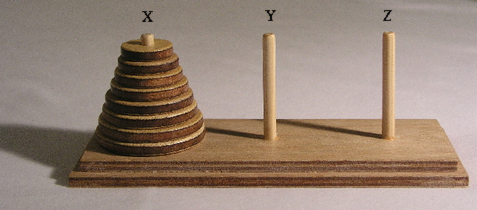
\includegraphics[width=180pt]{Tower-of-Hanoi.png}\\
\figcaption{Hanoi塔问题}\label{fig:hanoiTower}
\end{center}


现要求将X塔上的n个圆盘移动到Z上并仍按同样的顺序叠放,圆盘移动时必须遵循下列规则:
\begindot
\item 每次只能移动一个圆盘;
\item 圆盘可以插在X、Y和Z中的任一塔座上;
\item 任何时刻都不能将一个较大的圆盘压在较小的圆盘之上。
\myenddot
 
给出一个数$n$,求出最少步数的移动序列。


\subsubsection{输入}
一个整数 $n, n \leq 10$


\subsubsection{输出}
第一行一个整数$k$,表示最少的移动步数。

接下来$k$行,每行一句话,N from X to Y,表示把N号盘从X柱移动到Y柱。X,Y 属于\fn{\{'A','B','C'\}}


\subsubsection{样例输入}
\begin{Code}
3
\end{Code}


\subsubsection{样例输出}
\begin{Code}
7
1 from A to C
2 from A to B
1 from C to B
3 from A to C
1 from B to A
2 from B to C
1 from A to C
\end{Code}

\subsubsection{分析}
用递归。


\subsubsection{代码}

\begin{Codex}[label=hanoi.c]
#include <stdio.h>

/*
 * @brief 将塔座x上按直径有小到大且自上而下编号
 * 为1至n的n个圆盘按规则搬到塔座z上,y可用做辅助塔座.
 * @param[in] n 圆盘个数
 * @param[in] x 源塔座
 * @param[in] y 辅助塔座
 * @param[in] z 目标塔座
 * @return 无
 */
void hanoi(int n, char x, char y, char z) {
    if(n ==  1) {
        /* 将编号为n的圆盘从x移到z */
        printf("%d from %c to %c\n", n, x, z);
        return;
    } else {
        /* 将x上编号1至n-1的圆盘移到y,z作辅助塔 */
        hanoi(n-1, x, z, y);
        /* 将编号为n的圆盘从x移到z */
        printf("%d from %c to %c\n", n, x, z);
        /* 将y上编号1至n-1的圆盘移到z,x作辅助塔 */
        hanoi(n-1, y, x, z);
    }
}

int main() {
    int n;
    scanf("%d", &n);
    printf("%d\n", (1 << n) - 1); /* 总次数 */
    hanoi(n, 'A', 'B', 'C');
    return 0;
}
\end{Codex}


\subsubsection{相关的题目}
与本题相同的题目:
\begindot
\item wikioi 3145 汉诺塔游戏 , \myurl{http://www.wikioi.com/problem/3145/}
\myenddot

与本题相似的题目:
\begindot
\item  无
\myenddot


\subsection{进制转换}
\begin{Codex}[label=convert_base.cpp]
#include <stack>
#include <cstdio>

 /**
  * @brief 进制转换,将一个10进制整数转化为 d进制,d<=16.
  * @param[in] n 整数n
  * @param[in] d d进制
  * @return 无
  */
void convert_base(int n, const int d) {
    stack<int> s;
    int e;

    while(n != 0) {
        e = n % d;
        s.push(e);
        n /= d;
    }
    while(!s.empty()) {
        e = s.top();
        s.pop();
        printf("%X", e);
    }
    return;
}

const int MAXN = 64; // 栈的最大长度
int stack[MAXN];
int top = -1;
/**
 * @brief 进制转换,将一个10进制整数转化为 d进制,d<=16,更优化的版本.
 *
 * 如果可以预估栈的最大空间,则用数组来模拟栈,这时常用的一个技巧。
 * 这里,栈的最大长度是多少?假设CPU是64位,最大的整数则是2^64,由于
 * 数制最小为2,在这个进制下,数的位数最长,这就是栈的最大长度,最长为64。
 *
 * @param[in] n 整数n
 * @param[in] d d进制
 * @return 无
 */
void convert_base2(int n, const int d) {
    int e;

    while(n != 0) {
        e = n % d;
        stack[++top] = e; // push
        n /= d;
    }
    while(top >= 0) {
        e = stack[top--]; // pop
        printf("%X", e);
    }
    return;
}


/**
 * @brief 进制转换,将一个d进制整数转化为10进制,d<=16.
 * @param[in] s d进制整数
 * @param[in] d d进制
 * @return 10进制整数
 */
int restore(const char s[MAXN], const int d) {
    int result = 0;
    int one;

    for (int i = 0; s[i] != '\0'; i++) {
        if (s[i] >= '0' && s[i] <= '9') one = s[i] - '0';
        else if (s[i] >= 'A' && s[i] <= 'F') one = s[i] - 'A' + 10;
        else one = s[i] - 'a' + 10; /* (s[i] >= 'a' && s[i] <= 'f') */
        
        result = result * d + one;
    }
    return result;
}
\end{Codex}


\subsection{Design Queue by Stack}
Design a queue (FIFO) structure using only stacks (LIFO). 

Code is not necessary. 

Follow-up: provide a complexity analysis of push and remove operations.


\subsection{Valid Parentheses} %%%%%%%%%%%%%%%%%%%%%%%%%%%%%%
\label{sec:valid-parentheses}


\subsubsection{描述}
Given a string containing just the characters \code{'(', ')', '\{', '\}', '['} and \code{']'}, determine if the input string is valid.

The brackets must close in the correct order, \code{"()"} and \code{"()[]{}"} are all valid but \code{"(]"} and \code{"([)]"} are not.


\subsubsection{分析}
无


\subsubsection{代码}
\begin{Code}
	// LeetCode, Valid Parentheses
	// 时间复杂度O(n),空间复杂度O(n)
	class Solution {
		public:
		bool isValid (string const& s) {
			string left = "([{";
				string right = ")]}";
			stack<char> stk;
			
			for (auto c : s) {
				if (left.find(c) != string::npos) {
					stk.push (c);
				} else {
				if (stk.empty () || stk.top () != left[right.find (c)])
				return false;
				else
				stk.pop ();
			}
		}
		return stk.empty();
	}
};
\end{Code}


\subsubsection{相关题目}
\begindot
\item Generate Parentheses, 见 \S \ref{sec:generate-parentheses}
\item Longest Valid Parentheses, 见 \S \ref{sec:longest-valid-parentheses}
\myenddot


\subsection{Longest Valid Parentheses} %%%%%%%%%%%%%%%%%%%%%%%%%%%%%%
\label{sec:longest-valid-parentheses}


\subsubsection{描述}
Given a string containing just the characters \code{'('} and \code{')'}, find the length of the longest valid (well-formed) parentheses substring.

For \code{"(()"}, the longest valid parentheses substring is \code{"()"}, which has length = 2.

Another example is \code{")()())"}, where the longest valid parentheses substring is \code{"()()"}, which has length = 4.


\subsubsection{分析}
无


\subsubsection{使用栈}
\begin{Code}
	// LeetCode, Longest Valid Parenthese
	// 使用栈,时间复杂度O(n),空间复杂度O(n)
	class Solution {
		public:
		int longestValidParentheses(string s) {
			int max_len = 0, last = -1; // the position of the last ')'
			stack<int> lefts;  // keep track of the positions of non-matching '('s
			
			for (int i = 0; i < s.size(); ++i) {
				if (s[i] =='(') {
					lefts.push(i);
				} else {
				if (lefts.empty()) {
					// no matching left
					last = i;
				} else {
				// find a matching pair
				lefts.pop();
				if (lefts.empty()) {
					max_len = max(max_len, i-last);
				} else {
				max_len = max(max_len, i-lefts.top());
			}
		}
	}
}
return max_len;
}
};
\end{Code}

\subsubsection{Dynamic Programming, One Pass}
\begin{Code}
	// LeetCode, Longest Valid Parenthese
	// 时间复杂度O(n),空间复杂度O(n)
	// @author 一只杰森(http://weibo.com/wjson)
	class Solution {
		public:
		int longestValidParentheses(string s) {
			vector<int> f(s.size(), 0);
			int ret = 0;
			for (int i = s.size() - 2; i >= 0; --i) {
				int match = i + f[i + 1] + 1;
				// case: "((...))"
				if (s[i] == '(' && match < s.size() && s[match] == ')') {
					f[i] = f[i + 1] + 2;
					// if a valid sequence exist afterwards "((...))()"
					if (match + 1 < s.size()) f[i] += f[match + 1];
				}
				ret = max(ret, f[i]);
			}
			return ret;
		}
	};
\end{Code}


\subsubsection{两遍扫描}
\begin{Code}
	// LeetCode, Longest Valid Parenthese
	// 两遍扫描,时间复杂度O(n),空间复杂度O(1)
	// @author 曹鹏(http://weibo.com/cpcs)
	class Solution {
		public:
		int longestValidParentheses(string s) {
			int answer = 0, depth = 0, start = -1;
			for (int i = 0; i < s.size(); ++i) {
				if (s[i] == '(') {
					++depth;
				} else {
				--depth;
				if (depth < 0) {
					start = i;
					depth = 0;
				} else if (depth == 0) {
				answer = max(answer, i - start);
			}
		} 
	}
	
	depth = 0;
	start = s.size();
	for (int i = s.size() - 1; i >= 0; --i) {
		if (s[i] == ')') {
			++depth;
		} else {
		--depth;
		if (depth < 0) {
			start = i;
			depth = 0;
		} else if (depth == 0) {
		answer = max(answer, start - i);
	}
} 
}
return answer;
}
};
\end{Code}


\subsubsection{相关题目}
\begindot
\item Valid Parentheses, 见 \S \ref{sec:valid-parentheses}
\item Generate Parentheses, 见 \S \ref{sec:generate-parentheses}
\myenddot


\subsection{Largest Rectangle in Histogram} %%%%%%%%%%%%%%%%%%%%%%%%%%%%%%
\label{sec:largest-rectangle-in-histogram}


\subsubsection{描述}
Given $n$ non-negative integers representing the histogram's bar height where the width of each bar is 1, find the area of largest rectangle in the histogram.

\begin{center}
	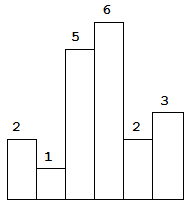
\includegraphics[width=120pt]{histogram.png}\\
	\figcaption{Above is a histogram where width of each bar is 1, given height = \fn{[2,1,5,6,2,3]}.}\label{fig:histogram}
\end{center}

\begin{center}
	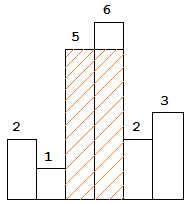
\includegraphics[width=120pt]{histogram-area.png}\\
	\figcaption{The largest rectangle is shown in the shaded area, which has area = 10 unit.}\label{fig:histogram-area}
\end{center}

For example,
Given height = \fn{[2,1,5,6,2,3]},
return 10.


\subsubsection{分析}
简单的,类似于 Container With Most Water(\S \ref{sec:container-with-most-water}),对每个柱子,左右扩展,直到碰到比自己矮的,计算这个矩形的面积,用一个变量记录最大的面积,复杂度$O(n^2)$,会超时。

如图\S 
\ref{fig:histogram-area}所示,从左到右处理直方,当$i=4$时,小于当前栈顶(即直方3),对于直方3,无论后面还是前面的直方,都不可能得到比目前栈顶元素更高的高度了,处理掉直方3(计算从直方3到直方4之间的矩形的面积,然后从栈里弹出);对于直方2也是如此;直到碰到比直方4更矮的直方1。

这就意味着,可以维护一个递增的栈,每次比较栈顶与当前元素。如果当前元素大于栈顶元素,则入栈,否则合并现有栈,直至栈顶元素小于当前元素。结尾时入栈元素0,重复合并一次。


\subsubsection{代码}
\begin{Code}
	// LeetCode, Largest Rectangle in Histogram
	// 时间复杂度O(n),空间复杂度O(n)
	class Solution {
		public:
		int largestRectangleArea(vector<int> &height) {
			stack<int> s;
			height.push_back(0);
			int result = 0;
			for (int i = 0; i < height.size(); ) {
				if (s.empty() || height[i] > height[s.top()])
				s.push(i++);
				else {
					int tmp = s.top();
					s.pop();
					result = max(result,
					height[tmp] * (s.empty() ? i : i - s.top() - 1));
				}
			}
			return result;
		}
	};
\end{Code}


\subsubsection{相关题目}
\begindot
\item Trapping Rain Water, 见 \S \ref{sec:trapping-rain-water}
\item Container With Most Water, 见 \S \ref{sec:container-with-most-water}
\myenddot


\subsection{Evaluate Reverse Polish Notation} %%%%%%%%%%%%%%%%%%%%%%%%%%%%%%
\label{sec:Evaluate-Reverse-Polish-Notation}


\subsubsection{描述}
Evaluate the value of an arithmetic expression in Reverse Polish Notation.

Valid operators are \fn{+, -, *, /}. Each operand may be an integer or another expression.

Some examples:
\begin{Code}
	["2", "1", "+", "3", "*"] -> ((2 + 1) * 3) -> 9
	["4", "13", "5", "/", "+"] -> (4 + (13 / 5)) -> 6
\end{Code}


\subsubsection{分析}
无


\subsubsection{递归版}
\begin{Code}
	// LeetCode, Evaluate Reverse Polish Notation
	// 递归,时间复杂度O(n),空间复杂度O(logn)
	class Solution {
		public:
		int evalRPN(vector<string> &tokens) {
			int x, y;
			auto token = tokens.back();  tokens.pop_back();
			if (is_operator(token))  {
				y = evalRPN(tokens);
				x = evalRPN(tokens);
				if (token[0] == '+')       x += y;
				else if (token[0] == '-')  x -= y;
				else if (token[0] == '*')  x *= y;
				else                       x /= y;
			} else  {
			size_t i;
			x = stoi(token, &i);
		}
		return x;
	}
	private:
	bool is_operator(const string &op) {
		return op.size() == 1 && string("+-*/").find(op) != string::npos;
	}
};
\end{Code}


\subsubsection{迭代版}
\begin{Code}
	// LeetCode, Max Points on a Line
	// 迭代,时间复杂度O(n),空间复杂度O(logn)
	class Solution {
		public:
		int evalRPN(vector<string> &tokens) {
			stack<string> s;
			for (auto token : tokens) {
				if (!is_operator(token)) {
					s.push(token);
				} else {
				int y = stoi(s.top());
				s.pop();
				int x = stoi(s.top());
				s.pop();
				if (token[0] == '+')       x += y;
				else if (token[0] == '-')  x -= y;
				else if (token[0] == '*')  x *= y;
				else                       x /= y;
				s.push(to_string(x));
			}
		}
		return stoi(s.top());
	}
	private:
	bool is_operator(const string &op) {
		return op.size() == 1 && string("+-*/").find(op) != string::npos;
	}
};
\end{Code}


\subsubsection{相关题目}
\begindot
\item 无
\myenddot


\section{队列} %%%%%%%%%%%%%%%%%%%%%%%%%%%%%%


\subsection{打印杨辉三角}

\begin{Codex}[label=yanghui_triangle.cpp]
#include <queue>
/**
 * @brief 打印杨辉三角系数.
 *
 * 分行打印二项式(a+b)^n展开式的系数。在输出上一行
 * 系数的同时,将其下一行的系数预先计算好,放入队列中。
 * 在各行系数之间插入一个0。
 *
 * @param[in] n (a+b)^n
 * @return 无
 */
void yanghui_triangle(const int n) {
    queue<int> q;
    /* 预先放入第一行的1 */
    q.push(1);

    for(int i = 0; i <= n; i++) {     /* 逐行处理*/
        int s = 0;
        q.push(s);      /* 在各行间插入一个0*/

        /* 处理第i行的i+2个系数(包括一个0)*/
        for(int j = 0; j < i+2; j++) {
            int t;
            int tmp;
            t = q.front();  /*读取一个系数,放入t*/
            q.pop();
            tmp = s + t;      /* 计算下一行系数,并进队列*/
            q.push(tmp);
            s = t;            /* 打印一个系数,第i+2个是0*/
            if(j != i+1) {
                printf("%d ",s);
            }
        }
        printf("\n");
    }
}
\end{Codex}
